\section{Gain saturation}

Gain saturation descirbes a phenomanon that occurs when the active region of a laser is unable to maintain its gain as the pump power increases for high values. 

To study this behavior, one measures the nonlinear behavior of the reflecitivty for an increasing amount of probe fluence, as can be seen in \cref{fig:gainSat}. To quantify this behavior and gain some macroscopic paramters, a model based on the saturation of the absorber in a SESAM can be fitted to the data. 

\begin{equation}
    \centering
    R(F)=R_{ns} \frac{F_{sat}}{F} \ln\left\{1 + \frac{R_{ss}}{R_{ns}} \left[\exp{ \left(\frac{F}{F_{sat}}\right) } - 1\right]\right\} \exp{\left(-\frac{F}{F_2}\right)}
    \label{eq:model}
\end{equation}

The parameters from \cref{eq:model} are the saturation fluence $F_{sat}$, the small signal reflictivity $R_{ss}$, the nonsaturable reflecitivty $R_{ns}$ and the rollover parameter $F_{2}$.

The saturation fluence $F_{sat}$ is the fluence at which the reflecitivity reduces to $1/e$ of its maximum. It also represents the point at which the population inversion inside the active region becomes saturated, therefore it is closely tied to the material properties of the active region.

The small signal reflecitivity $R_{ss}$ refers to the reflecitivty at low probe fleunce, where the gain is not significantly saturaed. In this regemie nonlinear effects are minimal and the reflectivity can be consiter the be in the linear regime and the small signal approximation can be applied and the small signal gain can be calcualted as $g_{ss}=R_{ss}-100\%$.

The nonsaturable reflectivity $R_{ns}$ arises from absorption and scattering at impurities and interfaces inside the VECSEL strucutre. This limits the maximum performance of the VECSE, thus reducing defect during the growing process is important. Since this effect is associated with imperfection and reflection inside the strucutre it remains relativily constand for different probe fluences. 

The rollover parameter $F_2$ describes further absorption from two photon absorption or higher order effects resulting in a strong decrease in the reflectivity at high fluences.

\Cref{fig:gainSat} shows the key parameters and the fitted model with and without accounting for the rollover for a measurement of a VECSEL with an integrated pump DBR.


\begin{figure}[ht]
    \centering
    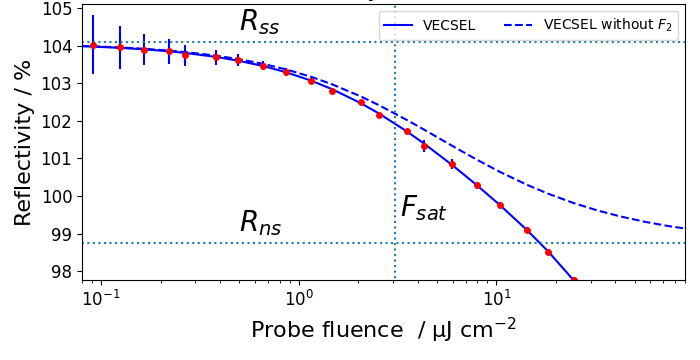
\includegraphics[width=12cm]{images/gainSat.png}
    \caption{Nonlinear reflectivity measurement for a diamond backed VECSEL with integrated pump DBR versus probe fluence. The data is shown with the fitted model utilizing \cref{eq:model} and the same model without the roll over paramter $F_2$. Additionally the different parameters $R_{ss}$, $R_{ns}$ and $F_{sat}$ are visualized.}
    \label{fig:gainSat}
\end{figure}